\documentclass[11pt,spanish]{report}

\usepackage{color}
\usepackage{listings}
\usepackage{amsmath}
\usepackage{graphicx}

\font\reallybigtenb=cmb10 scaled\magstep3
\parindent=0pt
\parskip=8.0pt
\baselineskip=12pt
\oddsidemargin=-0.5cm
\textwidth=17cm
\topmargin=-1.4cm
\textheight=23.0cm
\renewcommand{\arraystretch}{2}

\definecolor{codegreen}{rgb}{0,0.6,0}
\definecolor{codegray}{rgb}{0.5,0.5,0.5}
\definecolor{codepurple}{rgb}{0.58,0,0.82}
\definecolor{backcolour}{rgb}{0.95,0.95,0.92}
\lstdefinestyle{mystyle}{
    backgroundcolor=\color{backcolour},   
    commentstyle=\color{codegreen},
    keywordstyle=\color{magenta},
    numberstyle=\tiny\color{codegray},
    stringstyle=\color{codepurple},
    basicstyle=\ttfamily\footnotesize,
    breakatwhitespace=false,         
    breaklines=true,                 
    captionpos=b,                    
    keepspaces=true,                 
    numbers=none,                    
    numbersep=5pt,                  
    showspaces=false,                
    showstringspaces=false,
    showtabs=false,                  
    tabsize=2}
\lstset{style=mystyle}

\title{
    \begin{center}
        {\reallybigtenb{MTH1004}}
        
        {\reallybigtenb{Analysis of Atlantic Hurricanes and ENSO Effects}}
    \end{center}
}
\author{Jonas Brown}
\date{}

\usepackage[T1]{fontenc}
\usepackage{textcomp}
\usepackage{amstext}

\begin{document}

    \maketitle
    
    \chapter{Introduction}

    The purpose of this report is to investigate the relationship between the number of hurricanes in the Atlantic and the El Ni\~no Southern Oscillation (ENSO) index from 1870 to 2024. The end goal is to model hurricane counts using a probability distribution, see if ENSO influences hurricane frequency, and make predictions for the year to come.

    We were given a dataset consisting of three variables.
    
    \begin{itemize}
      \item Year (1870-2024),
      \item Number of hurricanes per year,
      \item ENSO index (temperature in \textdegree C).
    \end{itemize}

    From this dataset we have
    \begin{itemize}
        \item Total hurricane count: $n=155$,
        \item Mean hurricane count: $\bar{X}=1.79$,
        \item Variance of hurricane count: $\sigma^{2}=2.204$.
    \end{itemize}

    We are asked to choose a parametric model to describe the hurricane count and determine the impact of ENSO.

    \chapter{Modelling Hurricane Counts}

    \section{Potential Models}

    Hurricane count is a discrete, non-negative variable. This makes Poisson and Negative Binomial suitable models. A Poisson distribution assumes a constant variance; however, a Negative Binomial accounts for a variance that exceeds the mean. Using the Method of Moments, I will determine the best model out of the two.
    
    \section{Poisson Model}

    The Poisson distribution is defined as:

    \begin{center}
        \[ P(X=k|\lambda)=\frac{\lambda^{k}e^{-\lambda}}{k!}, \qquad k=0,1,2,... \]
    \end{center}

    where:

    \begin{itemize}
        \item \textbf{X} represents the number of hurricanes per year
        \item \boldmath$\lambda$ is the expected number of hurricanes per year
    \end{itemize}

    The Poisson distribution has the properties of

    \[E[X]=\lambda,\qquad Var(X)=\lambda\]

    Using the Method of Moments (MoM), we can estimate $\lambda$ by equating it to the sample mean.

    \[\hat{\lambda}_{MoM}=\bar{X}=1.79,\]

    \[SE(\lambda)=\sqrt{\frac{\lambda}{n}}=\sqrt{\frac{1.79}{155}}\approx0.11\]

    \section{Negative Binomial}

    The Negative Binomial distribution is potentially better than the Poisson model because it accounts for overdispersion. It has the properties of

    \[E[X]=\lambda=\frac{r(1-p)}{p},\qquad Var(X)=\lambda+\frac{\lambda^{2}}{r}\]

    If we rearrange for $r$ and then also $p$:

    \[\hat{r}=\frac{\lambda^{2}}{\sigma^{2}-\lambda},\qquad \hat{p}=\frac{r}{r+\lambda}\]

    Now, if we plug our numbers in:

    \[\hat{r}=\frac{1.79^{2}}{2.204-1.79}=\frac{3.2041}{0.414}\approx7.73,\]
    \[\hat{p}=\frac{7.74}{7.74+1.79}=\frac{7.74}{9.53}\approx0.811\]

    \[Var(\mu)=\frac{\sigma^{2}}{n}=\frac{2.204}{155}\]
    \[SE(\mu)=\sqrt{\frac{2.204}{155}}\approx0.12\]

    \section{Conclusion}

    The Negative Binomial model better for this data as it accounts for overdispersion (variance > mean). The Poisson distribution assumes that $Var(X)=\lambda$, however the observed variance ($2.204$) is greater than the mean ($1.79$), which indicates overdispersion. The Negative Binomial model has an additional parameter $r$ to handle this and should be used instead of the Poisson model.

    \subsection{Parameters}

    The high value of $r$ suggests that the data is closer to a Poisson distribution than a Negative Binomial. However, the high value of $p$ (success probability in the Negative Binomial model) is consistent with the low hurricane counts.

    \subsection{Errors}
    
    The standard error for the Negative Binomial model is slightly larger than that for the Poisson, which reflects the adjusted variance estimate. The standard error depends on both $r$ and $\lambda$, but the impact is unnoticeable here as the value of $r$ is so high. 

    \subsection{Realism}

    The Negative Binomial model is a better choice due to its flexibility in modelling variance. The estimate for $r\approx7.73$ is rather large for a typical case of overdispersion, however with this data it is reasonable to assume the model is a Negative Binomial still. To add to this, an even larger $r$ value would start to suggest the model is Poisson. In addition, the parameter $p\approx0.811$ suggests that the success probability is quite high, which seems correct for hurricanes.

    \subsection{Visual Representation}

    As you can see from the figure below, the Negative Binomial model fits the extremes better than the Poisson. It also, generally, follows the shape of the observed frequencies better too.

    \begin{center}
        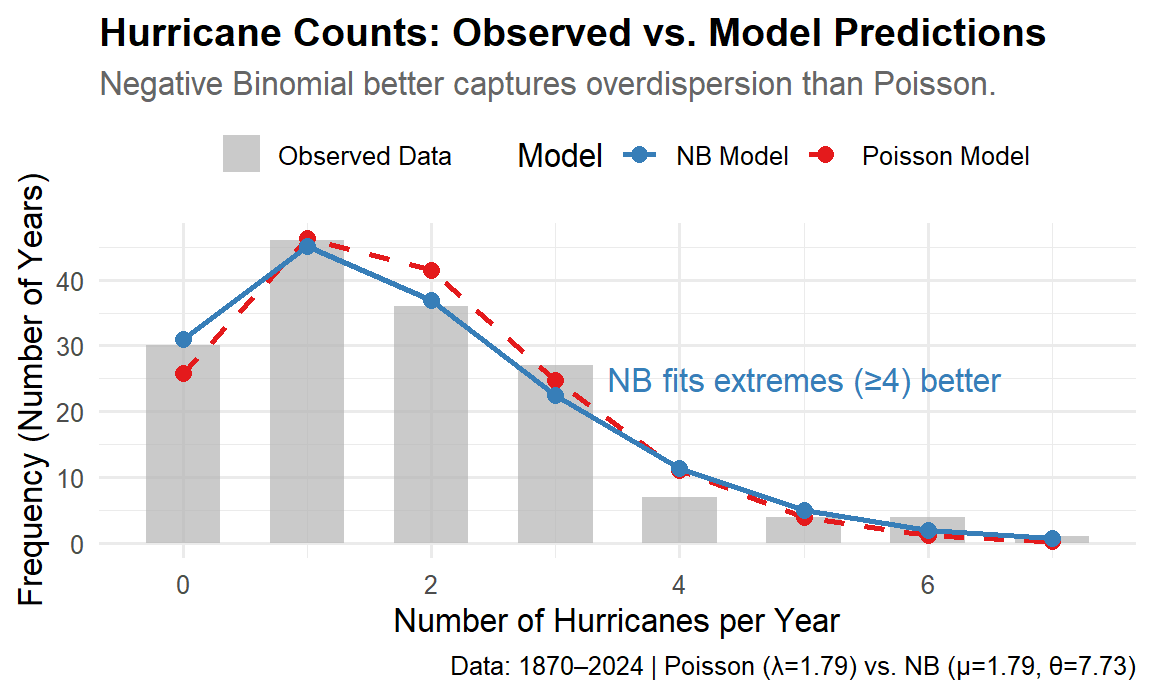
\includegraphics[width=0.75\linewidth]{observed_vs_models}
    \end{center}

    \chapter{Impact Of ENSO On Hurricanes}

    Dividing the ENSO index data into two groups (negative and neutral/positive), we can compare the expected number of hurricanes and assess whether the hurricane count changes with the sign of the ENSO index.

    Since we're using a Negative Binomial distribution our variance and standard error will be
    
    \[Var(X_{\pm})=\hat{\mu}_{\pm}+\frac{\hat{\mu}_{\pm}^{2}}{r}\]
    \[SE(\mu_{\pm})=\sqrt{Var(\mu_{\pm})}\]

    Furthermore, since I'll be using a 95\% Critical Interval, our $z_{0.025}=1.96$.

    \begin{center}
        \begin{tabular}{ |c|c|c|c|c|c| } 
            \hline
            Group & Years & Mean & Variance & Standard Error & 95\% Confidence Interval \\
            \hline
            Negative & $97$ & $2.09$ & $2.655$ & $0.166$ & $2.09\pm1.96\times0.166\approx(1.76,2.42)$ \\
            \hline
            Neutral/Positive & $58$ & $1.29$ & $1.505$ & $0.158$ & $1.29\pm1.96\times0.158\approx(0.98,1.60)$ \\
            \hline
        \end{tabular}
    \end{center}

    So, we have all our information. Let's now assess whether
    the expected number of hurricanes changes with the sign of the ENSO index.

    Let's use a Z-test to do this:

    \[H_{0}: \mu_{-}=\mu_{+},\qquad H_{1}: \mu_{-}>\mu_{+}\]
    
    \[Z=\frac{\mu_{-}-\mu_{+}}{\sqrt{SE(\mu_{-})^{2}+SE(\mu_{+})^{2}}}=\frac{2.09-1.29}{\sqrt{0.166^{2}+0.158^{2}}}\approx3.42\]
    
    \[p=P(Z<3.42)<0.001\]

    The p-value calculated provides strong evidence to reject $H_{0}$, suggesting the expected number of hurricanes changes with the sign of the ENSO index.
    
    \[\text{Incidence Rate Ratio}=\frac{\mu_{-}}{\mu_{+}}=\frac{2.09}{1.29}\approx1.62\]

    Using the Incidence Rate Ratio, we can say that negative ENSO index years have 62\% more hurricanes on average. This aligns with meteorological theory that cooler Pacific temperatures (negative ENSO) benefit hurricane formation.
    
    \chapter{Predicting 2025}

    \section{Prediction Interval}

    For a Negative Binomial distribution the approximate prediction interval for 2025 is

    \[\text{PI}=\mu\pm z_{0.95}\sqrt{\mu+\frac{\mu}{r}}\]

    where:

    \begin{itemize}
        \item $\mu=1.79$
        \item $r=7.73$
        \item $z_{0.95}=1.645$ (two-tailed so we only need 5\%)
    \end{itemize}

    \[\sigma=\sqrt{1.79+\frac{1.79^{2}}{7.73}}\approx1.79+0.414\approx1.486\]
    \[\text{PI}=1.79\pm1.645\times\sigma\approx1.79\pm2.44\approx(-0.65,4.23)\]

    Since hurricane counts cannot be negative, we set the lower bound to 0. This gives us $[0,4]$ as our prediction interval.

    \section{Three Or More Hurricanes In 2025?}

    Let's find out how likely it is for there to be 3 or more hurricanes in 2025...

    \[P(X\geq3)=1-P(X\leq2)=1-[P(X=0)+P(X=1)+P(X=2)]\]

    After writing some basic R code to work this out, I got
    
    \[P(X\geq3)\approx27.12\%\]

    I would conclude that 3 or more hurricanes in 2025 are fairly unlikely to happen, since we have quite a low probability.

    \section{Trustworthiness}

    \subsection{Strengths}

    \begin{itemize}
        \item The Negative Binomial model accounts for overdispersion in hurricane counts (variance > mean), providing more realistic uncertainty estimates than the Poisson model.
        \item ENSO index groups (positive/negative) align with known climate science.
    \end{itemize}

    \subsection{Limits}

    \begin{itemize}
        \item The model assumes future hurricane behavior will continue as recorded - climate change may affect ENSO-hurricane relationships, reducing reliability for future predictions.
        \item The dispersion parameter is estimated from historical data. 
        \item The model treats annual hurricane counts independently.
    \end{itemize}

    \subsection{Conclusion}

    The statistical model is perfect for short-term, stationary conditions. But, it should be climate-adjusted for longer-term predictions.

    \section{A Climate Scientist Tells Us...}

    We are told that a climate scientist says that "the probability of the ENSO index being positive in 2025 is $0.25$." What does this mean for our probability prediction?

    Let's compute $P(X\geq3)$:

    \[\text{Using }P(X\geq3)=1-P(X\leq2)\text{ from earlier.}\]
    \[P(X\geq3|\text{ENSO}_{+})\approx0.1521\]
    \[P(X\geq3|\text{ENSO}_{-})\approx0.3437\]

    Given $P(\text{ENSO}_{+})=0.25$ we also have $P(\text{ENSO}_{-})=0.75$.

    So, overall, the total probability is

    \[P(X\geq3)\approx(0.1521\times0.25)+(0.3437\times0.75)=0.2958=29.58\%\]

    \subsection{New Conclusion}

    The probability increases by only 2.5\% (from 27.1\% to 29.6\%) due to the 75\% chance of negative ENSO conditions. This small increase shows the overdispersion in hurricane counts (which dampens the impact of variance in the ENSO index) and the smaller than expected difference between ENSO index groups.
 

    

\end{document}
